\documentclass[glossy]{beamer}
\useoutertheme{wuerzburg}
\useinnertheme[realshadow,corners=2pt,padding=2pt]{chamfered}
\usecolortheme{shark}

\usepackage{listings}

\usepackage{tikz}
\newcommand<>{\hover}[1]{\uncover#2{%
 \begin{tikzpicture}[remember picture,overlay]%
 \draw[fill,opacity=0.4] (current page.south west)
 rectangle (current page.north east);
 \node at (current page.center) {#1};
 \end{tikzpicture}}
}

\title{Arquitecturas y Organización de Computadoras I \\\line(1,0){320}}
% \author{\texorpdfstring{Author\newline\url{email@email.com}}{Author}}
%\author{Rafael Ignacio Zurita}
\institute{Rafael Ignacio Zurita \\ Departamento de Ingenieria de Computadoras - FAI - UNCOMA 2018 \\ Clase presencial 2}
%\date{\today}



\begin{document}




\begin{frame}
\maketitle
\end{frame}

\institute{Departamento de Ingenieria de Computadoras - FAI - UNCOMA \\ 2018}

\begin{frame}
\frametitle{Programa Analítico}
\textbf{UNIDAD I: Arquitectura y Organización de Computadoras}
 \\~\\
\textit{Organización  funcional. Repaso del modelo de Von Neumann. Concepto de Arquitectura y Organización de Computadoras. Representación de datos a nivel de máquina. Direccionamiento de memoria: concepto de palabra, ordenamiento de bytes. Registros.} 
 \\~\\
Formatos de Instrucciones. Modos de direccionamiento. Tipos de instrucciones: transferencia de datos, operaciones aritméticas y lógicas, transferencia de control. Excepciones. Lenguaje ensamblador: directivas, operaciones, pseudo-operaciones, macros.
\end{frame}


\begin{frame}
\frametitle{Arquitecturas y Organización de Computadoras}
\textbf{Modelo he programación}
\textit{Para programar una computadora se debe comprender la memoria interna de la CPU (registros), su conjunto de instrucciones, y sus modos de direccionamiento.}
\end{frame}


\begin{frame}
\frametitle{Arquitecturas y Organización de Computadoras}
\textbf{Repaso de conceptos}
\begin{itemize}
	\item  \textbf{Arquitectura}: (tambien ISA: instruction set architecture) Los componentes del diseño del procesador 
que necesitan ser comprendidos para programar una computadora.
Ejemplos: especificacion del conjunto de instrucciones, registros, modos de direccionamiento.
\item  \textbf{Microarquitectura}: Implementación de la Arquitectura.
Ejemplos: ejecución out-of-order, pipeling, ejecución especulativa, tamaño de caches, frecuencia del reloj.
\item \textbf{Ejemplos de ISAs}: x86, IA, MIPS, ARM, SPARC, SUPERH, VAX, 68000, AVR

\end{itemize}
\end{frame}



\begin{frame}
	\textbf{Architecture vs. Microarchitecture} \\	
\begin{itemize}
	\item	\textit{Arquitectura (Instruction Set Architecture):}	
\begin{itemize}
	\item Estado visible al programador (memoria y registros)
	\item Operaciones (Instrucciones, y sus acciones)
	\item Semántica de ejecución (interrupciones)
	\item Entrada/Salida
	\item Tipos de datos (tamaños)
\end{itemize}
\item	\textit{Organizacion (Microarquitectura):}	
\begin{itemize}
	\item Compromiso en como implementar un ISA para alguna métrica (rendimiento, consumo, costo)
\item Ejemplos: profundidad del pipeling,  número de pipelings, tamaño de caches, área del chip, potencia pico, orden de ejecución, ancho de bus, ancho de la ALU
\end{itemize}
\end{itemize}
\end{frame}


\begin{frame}
\frametitle{Historia del concepto Arquitectura}
	\begin{itemize}

		\item	\textbf{Problema de compatibilidad de IBM} \\
	Durante 1960's, IBM tuvo 4 líneas de computadoras incompatibles!
	\begin{itemize}
		\item 701 ⇒ 7094
		\item 650 ⇒ 7074
		\item 702 ⇒ 7080
		\item 1401 ⇒ 7010 
	\end{itemize}
	\end{itemize}
\end{frame}

\begin{frame}
\frametitle{Historia del concepto Arquitectura}
	\begin{itemize}
		\item\textbf{Problema de compatibilidad de IBM} \\
	Durante 1960's, IBM tuvo 4 líneas de computadoras incompatibles!
	\begin{itemize}
		\item 701 ⇒ 7094
		\item 650 ⇒ 7074
		\item 702 ⇒ 7080
		\item 1401 ⇒ 7010
	\end{itemize}
\item \textit{Cada sistema tuvo su propio}
	\begin{itemize}
		\item Conjunto de instrucciones
		\item Sistema de E/S y almacenamiento secundario (cintas magnetica, tambores y discos)
		\item ensambladores, compiladores, bibliotecas
		\item diferentes mercados: científico, comercial/bancario, tiempo real
	\end{itemize}
	\end{itemize}
\end{frame}

\begin{frame}
\frametitle{Historia del concepto Arquitectura}
	\begin{itemize}
		\item\textbf{Problema de compatibilidad de IBM} \\
	Durante 1960's, IBM tuvo 4 líneas de computadoras incompatibles!
	\begin{itemize}
		\item 701 ⇒ 7094
		\item 650 ⇒ 7074
		\item 702 ⇒ 7080
		\item 1401 ⇒ 7010
	\end{itemize}
\item \textit{Cada sistema tuvo su propio}
	\begin{itemize}
		\item Conjunto de instrucciones
		\item Sistema de E/S y almacenamiento secundario (cintas magnetica, tambores y discos)
		\item ensambladores, compiladores, bibliotecas
		\item diferentes mercados: científico, comercial/bancario, tiempo real
	\end{itemize}
\item	\textbf{ Respuesta de IBM: ==⇒ IBM	360 == }
	\end{itemize}
\end{frame}






\begin{frame}
\frametitle{IBM 360}
\begin{figure}
\includegraphics[scale=0.2]{IBM-360.jpg} 
\caption{Implementaciones iniciales del IBM 360}
\label{Implementacione Iniciales del IBM 360}
\end{figure}

	\begin{itemize}
	\item Estado del procesador: 16 registros de 32-bit de propósito general, 4 de punto flotante, PC, flags
	\item Arquitectura de 32-bits con direcciones de 24 bits
	\item Formato de datos: bytes de 8-bits, palabra de 32-bits, half y double
	\item \textbf{Primera familia de computadoras con un mismo ISA} 
	\end{itemize}
\end{frame}


\begin{frame}
\frametitle{Programación de la máquina}
	\textbf{Modelo de programación (Arquitectura)}
\begin{figure}
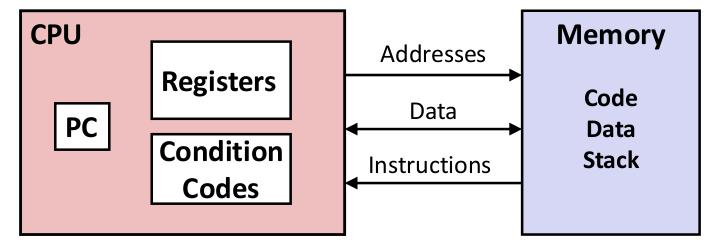
\includegraphics[scale=0.3]{componentes-CPU.jpg} 
\caption{Componentes de la máquina}
\label{Componentes de la máquina}
\end{figure}
	\textit{Estado visible al programador}
	\begin{itemize}
		\item \textbf{Registros} PC, propósito general, stack pointer\\
		\item \textbf{Memoria}: arreglo direccionable por byte. Codigo y datos de usuario. Pila y memoria dinamica
	\end{itemize}
\end{frame}


\begin{frame}
\frametitle{Programación de la máquina}
\textbf{Modelo de programación (Arquitectura)}
\begin{tabular}{cl}

\begin{tabular}{c}
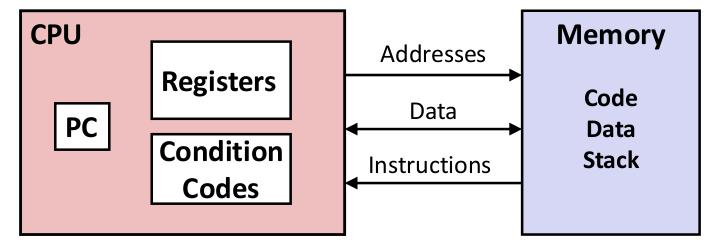
\includegraphics[height=5cm, width=4.5cm]{componentes-CPU.jpg} 

\end{tabular}
& \begin{tabular}{l}
\parbox{0.5\linewidth}{

\textbf{Registros} PC, propósito general, stack pointer\\
\textbf{Memoria}: arreglo direccionable por byte. Codigo y datos de usuario. Pila y memoria dinamica
}
\end{tabular} \\

\end{tabular}
\end{frame}
 


\begin{frame}
	
\begin{tabular}{cl}

\begin{tabular}{c}
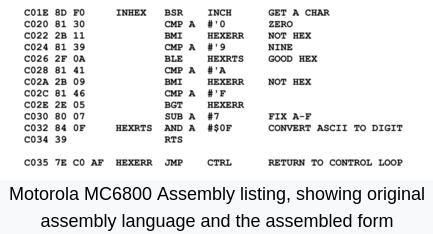
\includegraphics[height=5cm, width=4.5cm]{assembly.jpg} 
\end{tabular}
& \begin{tabular}{l}
\parbox{0.5\linewidth}{

\textbf{Etiqueta} pero la pucha que vale la pena estar vivo \\
\textbf{Instruccion} pero la pucha que vale la pena estar vivo \\
\textbf{Operandos} pero la pucha que vale la pena estar vivo \\
\textbf{Comentarios} pero la pucha que vale la pena estar vivo 
}
\end{tabular} \\

\end{tabular}


\end{frame}





% INDICE: HISTORIA de procesadores y arquitectura (filmina de arquitectura de david), system 360, zseries, 
% compilacion, ensamblado, codigo maquina
% ejemplo x86 , uso de longitud variable para instruccciones, instrucciongs con dos operandos, pocos registros, infinidad de modos de direccion2miento para cada operacion. En cada version nuevas instrucciones y compatibilidad. Cientos de instrucciones CISC
% Microarquitectura : programada (interprete), en hardware
% grafico inicio de RISC: quitar el interprete, hacer un set sencillo, fijo y de pocos formatos
% limite de energia, nacimiento de arquitecturas avanzadas 
%
% lenguaje ensamblador, figura de compilacion, ejemplo de ensamblador x86, figura de dos arquitecturas x86, system 360, zseries,X , filmina de diferencia entre arquitectura y organizacion, estructura por capas y resumen de los temas a ver en la materia,  memoria, 
% segunda parte: antes de ver lenguaje ensamblador veremos terminologia importante sobre la organizacion  de la memoria
% Representación de datos a nivel de máquina. Direccionamiento de memoria: concepto de palabra, ordenamiento de bytes. Registros.} 
% memori2, direccion, byte, palabra, alineacion, endianess, instrucciones y datos
% directivas MIPS, etc para el practico

\begin{frame}
\frametitle{Computadora}

x86 assembly language is a family of backward-compatible assembly languages, which provide some level of compatibility all the way back to the Intel 8008 introduced in April 1972. x86 assembly languages are used to produce object code for the x86 class of processors. Like all assembly languages, it uses short mnemonics to represent the fundamental instructions that the CPU in a computer can understand and follow. Compilers sometimes produce assembly code as an intermediate step when translating a high level program into machine code. Regarded as a programming language, assembly coding is machine-specific and low level. Assembly languages are more typically used for detailed and time critical applications such as small real-time embedded systems or operating system kernels and device drivers.
%\begin{figure}
%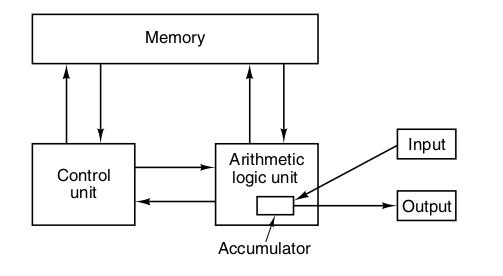
\includegraphics[scale=0.5]{maq-von-neumann.jpg} 
%\caption{Modelo de Von Neumann}
%\label{Modelo de Von Neumann}
%\end{figure}
% ¿programa-almacenado?
\end{frame}
 
 
 
 

\begin{frame}
\frametitle{Organización de computadora estructurada}
\begin{itemize}
\item Lenguaje de alto nivel
\item Lenguaje ensamblador
\begin{itemize}
\item Lenguaje de alto nivel
\item Lenguaje ensamblador
\end{itemize}
\item ISA
\end{itemize}
\end{frame}

\begin{frame}
\frametitle{Arquitecturas y Organización de Computadoras}
¿Por qué estudiar todos estos conceptos?
\begin{itemize}
\item Tiempo de Ejecución de programas
\item Control de riego / laboratorio
\item Prestaciones - Multiprocesadores - Arquitecturas avanzadas - Consumo
\end{itemize}
\end{frame}

\begin{frame}
\frametitle{Arquitecturas y Organización de Computadoras}
Clases de computadoras
\begin{itemize}
\item PC - workstation
\item Servidor
\item Cluster
\item SuperComputadora (cientos de miles de procesadores, terabytes, petabytes)
\item Sistemas embebidos
\end{itemize}
\end{frame}
 

\begin{frame}
 \frametitle{Consejos y preguntas}
\begin{center}
\begin{itemize}
\item  ¿Preguntas?
\end{itemize}
\end{center}
\end{frame}


\begin{frame}
 \frametitle{Bibliografía}
Libros
\begin{itemize}
\item Andrew S. Tanenbaum (2000), ORGANIZACIÓN DE COMPUTADORAS un enfoque estructurado, Editorial Prentice Hall. (10 copias en biblioteca)
\item David. Patterson John L. Hennessy (1995), ORGANIZACIÓN Y DISEÑO DE COMPUTADORES La interfaz hardware/software, McGraw-Hill (8 copias en biblioteca).
\end{itemize}
Contenido electrónico
\begin{itemize}
	\item \textbf{x86 assembly basis} Una introducción al lenguaje ensamblador x86. Disponible en PEDCO en formato PDF.
		\url{https://www.nayuki.io/page/a-fundamental-introduction-to-x86-assembly-programming}
\item Apuntes elaborados por la cátedra, disponibles en PEDCO para impresión (pdf) o lectura online (html)
\item Secciones de libros aptas para publicacion
\end{itemize}
\end{frame}


\end{document}
